\documentclass[a4paper, 14pt]{extarticle}%тип документа

%Русский язык
\usepackage[T2A]{fontenc} %кодировка
\usepackage[utf8]{inputenc} %кодировка исходного кода
\usepackage[english,russian]{babel} %локализация и переносы

%отступы 
\usepackage[left=2cm,right=2cm,top=2cm,bottom=3cm,bindingoffset=0cm]{geometry}

%Вставка картинок
\usepackage{graphicx}
\usepackage{wrapfig, caption}
\graphicspath{}
\DeclareGraphicsExtensions{.pdf,.png,.jpg, .jpeg}
\newcommand\ECaption[1]{%
     \captionsetup{font=footnotesize}%
     \caption{#1}}

%Таблицы
\usepackage[table,xcdraw]{xcolor}
\usepackage{booktabs}

%Графики
\usepackage{pgfplots}
\pgfplotsset{compat=1.9}

%Математика
\usepackage{amsmath, amsfonts, amssymb, amsthm, mathtools}

%Заголовок
\author{Подлесный Артём \\ группа 827}
\title{Работа 1.2 \\ Исследование эффекта Комптона}

\begin{document}
\maketitle

\section*{Экспериментальная установка}

\begin{figure}[h]
\begin{center}
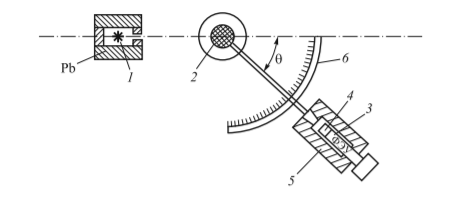
\includegraphics[width=0.9\textwidth]{ust}
\end{center}
\ECaption{Блок-схема по изучению рассеяния $\gamma$-квантов.}
\end{figure}

Эффект Комптона представляет собой один из простейших способов убедиться в дуальной природе частиц. Для энергий он записывается в следующем виде:
\begin{equation}
\frac{1}{\varepsilon(\theta)}-\frac{1}{\varepsilon_0} = 1-\cos\theta,
\end{equation}
где $\varepsilon = \frac{E}{mc^2}$ -- приведенная энергия $\gamma$-кванта, рассеянного и покоющегося соответственно.

В условиях эксперимента можно было изменять угол до 120$^{\circ}$. Кванты, испытавшие рассеяние под углом, на который установлен счетчик, можно исследовать с помощью установки. Сам счетчик выводит сигналы, связанные не с самими $\gamma$-квантами, а с образовавшимися под их действием в кристалле электроны. Над сигналом проводится амплитудный анализ по импульсам, благодаря чему каждому импульсу электрона соответствует собственный канал (с некоторой точностью). Гистограмма числа отсчетов от номера канала выводится на экран, как на рис.2:

\begin{figure}[h]
\begin{center}
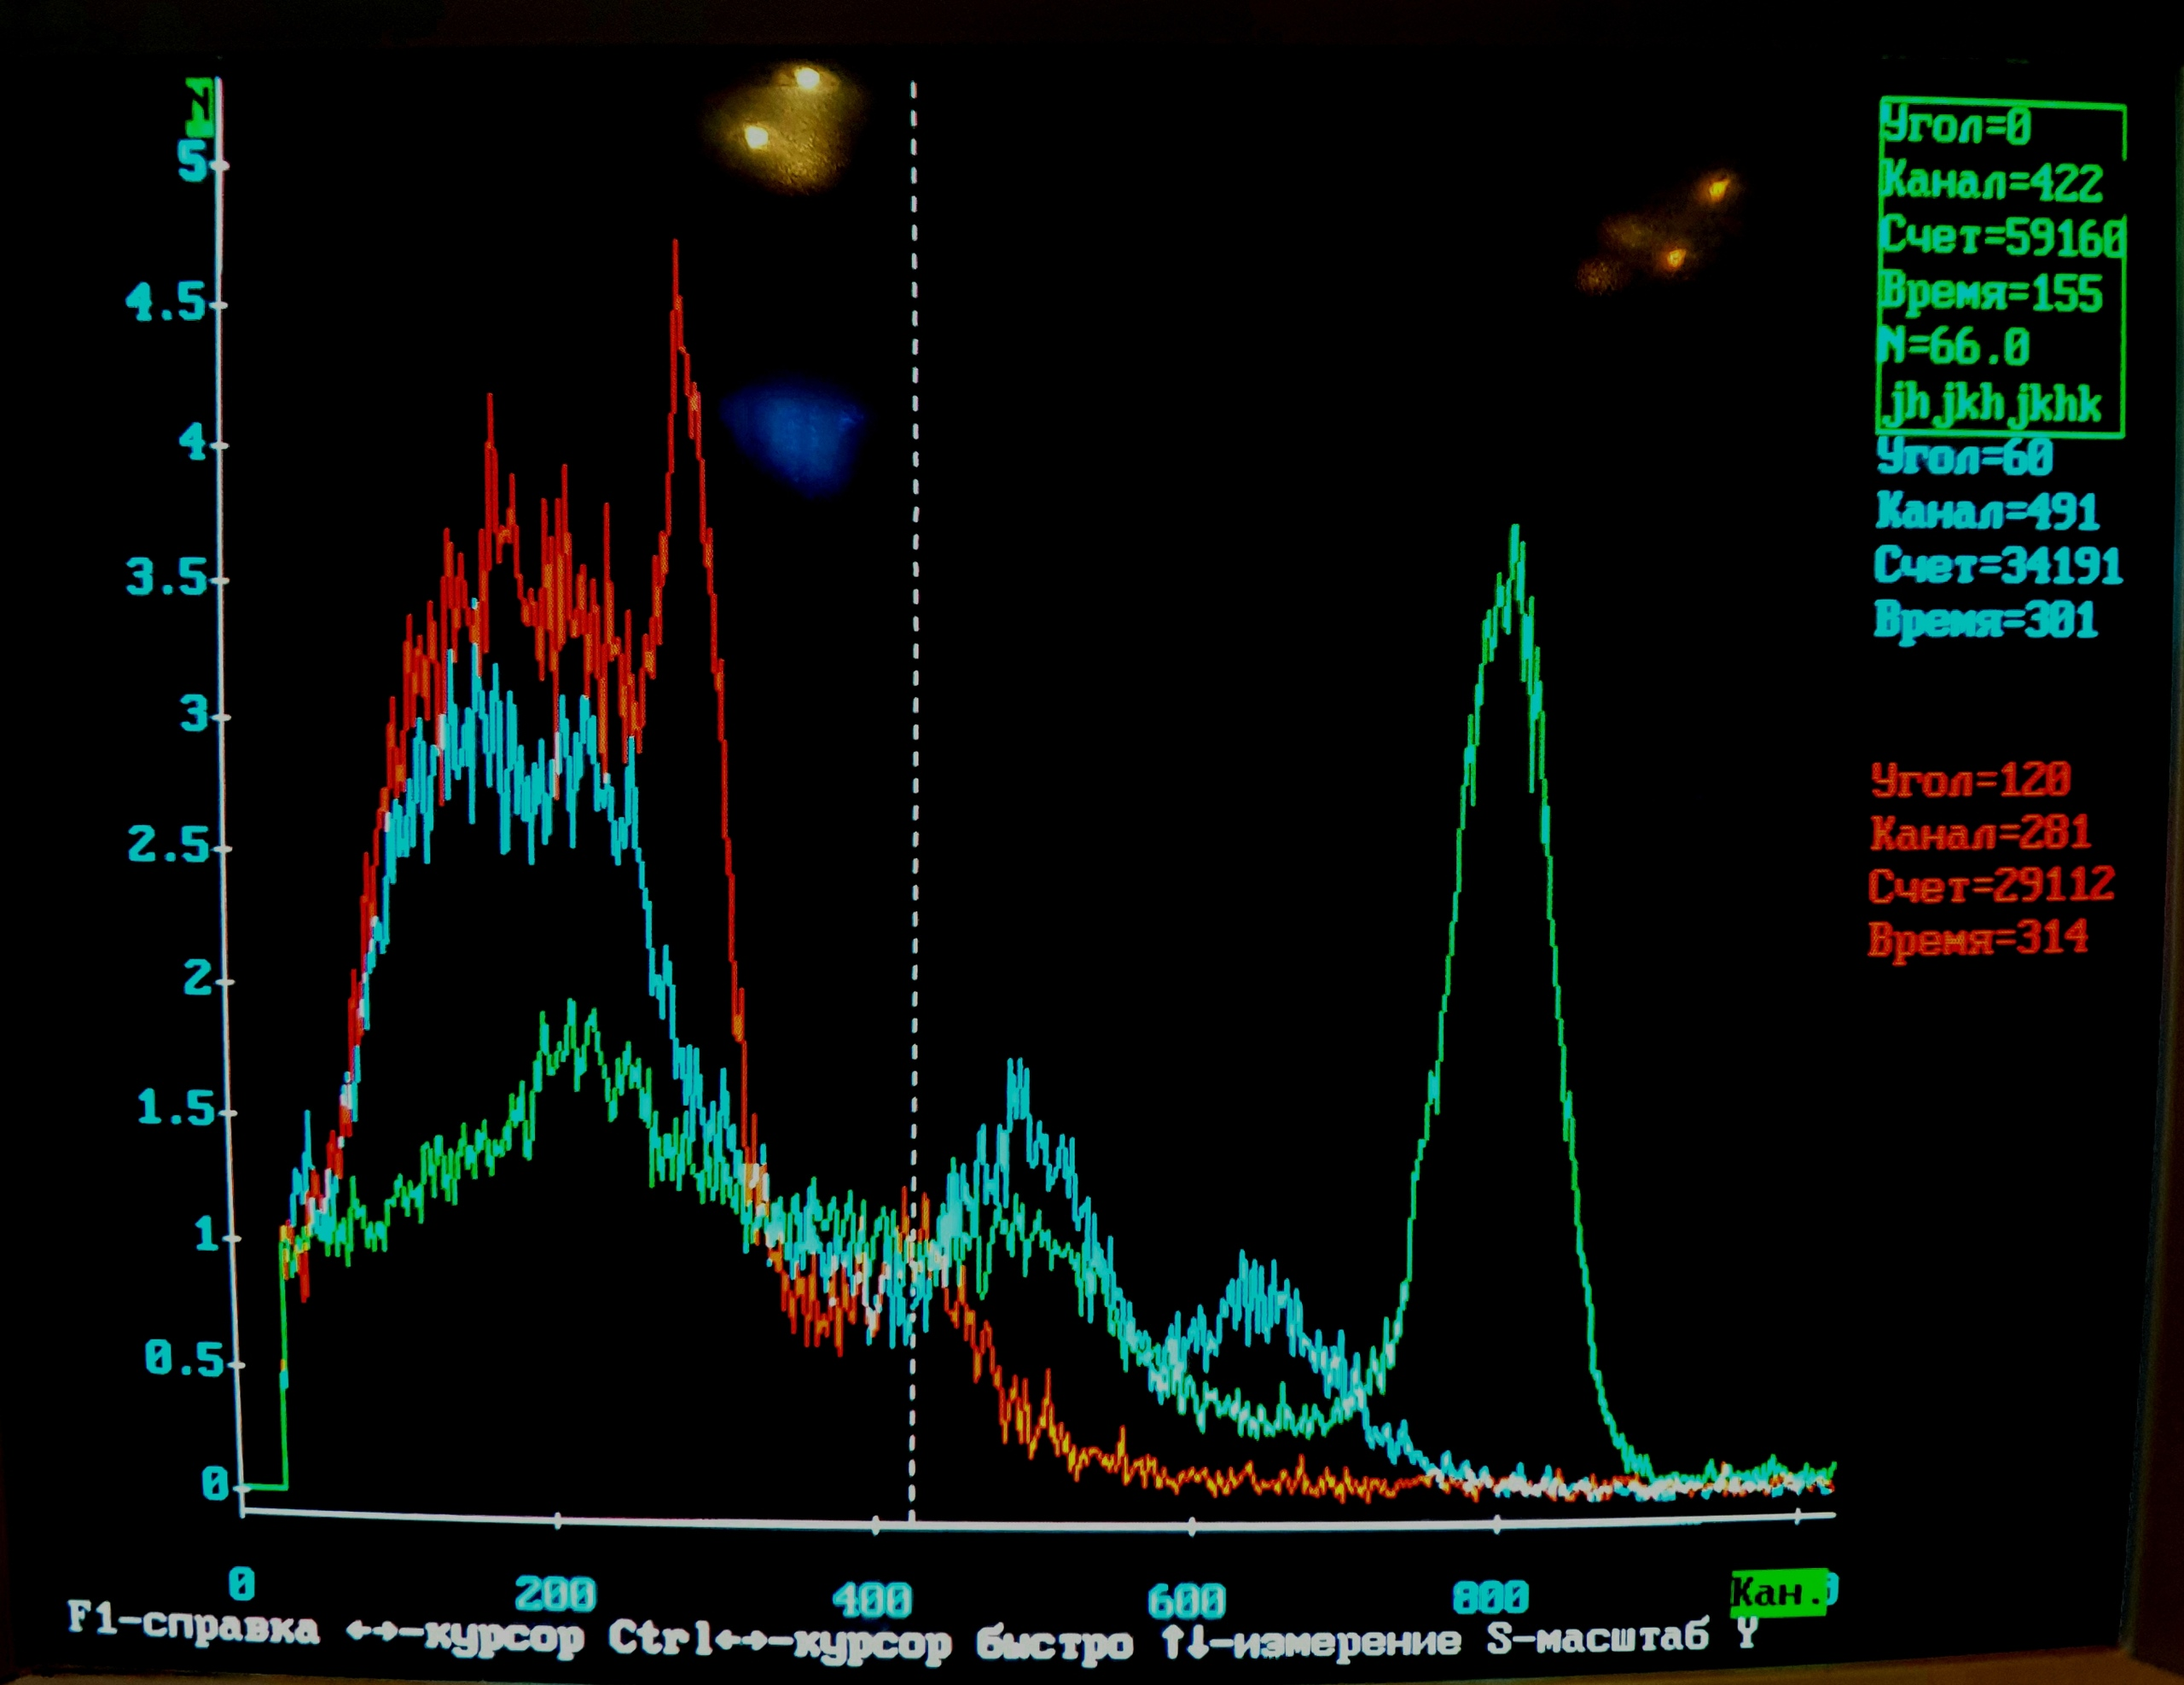
\includegraphics[width=0.7\textwidth]{gys}
\end{center}
\ECaption{Гистограмма сигналов сразу нескольких измерений. Четко видны фотопики, а так же зависимость положения пиков от угла измерения, что соотвествует зависимости положения пика от энергии $\gamma$-квантов. }
\end{figure}

Так как при фотоэффекте $\gamma$-квант полностью поглощается, то положение пика соответсвует энергии самого кванта. Так же кванты могут испытавать комптоновское рассеяние на свободных электронах, из-за чего появляется непрерывный аплитудный спектр электронов до самого фотопика.

Ширина пика связана со строением установки и кристалла, так что не влияет на результат. Так же на больших углах могут наблюдаться второй и третий пики. Это происходит из-за того, что при низкий энергиях кванты могут испытывать повторное рассеяние, из-за чего количество быстрых электронов увеличивается, и за время измерения они возбуждают большее количество атомов ФЭУ, из-за чего число вспышек увеличивается. Это тоже является артефактом установки, так что при измерениях нужно учитывать только вершину первого пика.

\section*{Энергия покоя частицы, на которой происходит рассеяние}

Из формулы (1) и описания работы установки получаем формулу для экспериментальных данных:
\begin{equation}
\frac{1}{N(\theta)} - \frac{1}{N_0} = A(1-\cos\theta),
\end{equation}
где $N$ -- номер канала, на котором находится вершина пика, $A$ -- коэффициент пропорциональности между $N$ и $\varepsilon$. Результаты измерений представлены на таблице 1.

\begin{table}[h!]
\begin{center}
\begin{tabular}{|c|c|c|}
\hline
\rowcolor[HTML]{9698ED} 
$\theta$, $^{\circ}$ & $N$ & $t$, сек \\ \hline
0                    & 690 & 303      \\ \hline
\rowcolor[HTML]{9698ED} 
10                   & 820 & 275      \\ \hline
20                   & 763 & 372      \\ \hline
\rowcolor[HTML]{9698ED} 
30                   & 713 & 277      \\ \hline
40                   & 643 & 218      \\ \hline
\rowcolor[HTML]{9698ED} 
50                   & 545 & 484      \\ \hline
60                   & 491 & 301      \\ \hline
\rowcolor[HTML]{9698ED} 
70                   & 432 & 237      \\ \hline
80                   & 391 & 250      \\ \hline
\rowcolor[HTML]{9698ED} 
90                   & 354 & 281      \\ \hline
100                  & 327 & 329      \\ \hline
\end{tabular}
\ECaption{Зависимость $N(\theta)$. На данной установке была возможность измерять только в диапазоне $0\div100^{\circ}$. }
\end{center}
\end{table}

По этим данным построен линеаризованый график, представленный на рис.3.
\begin{figure}[h]
\begin{center}
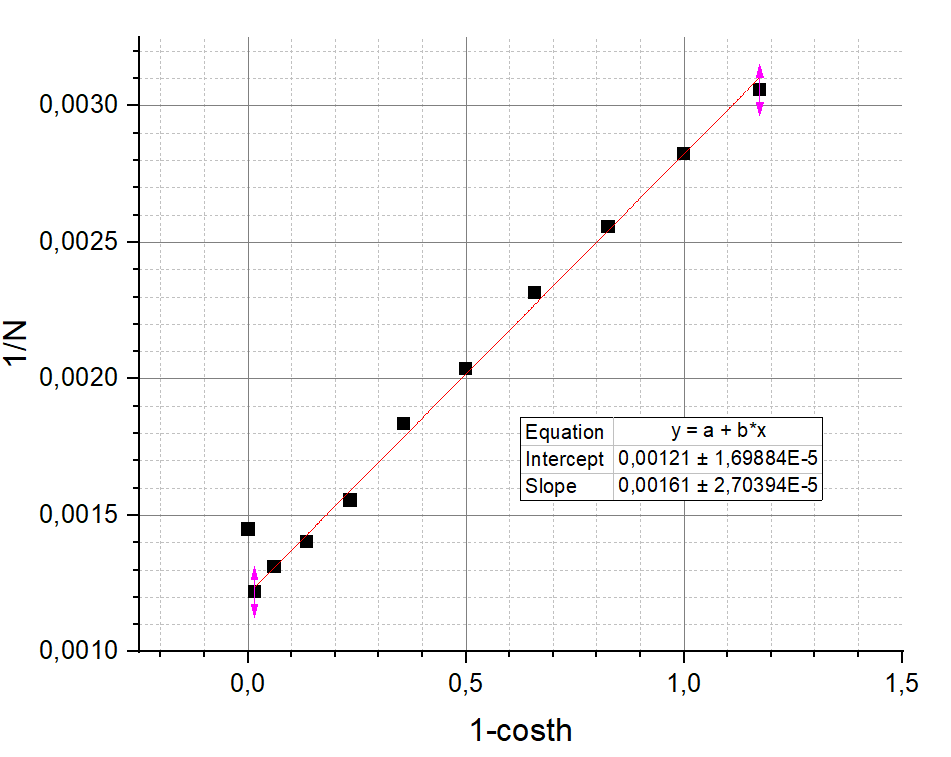
\includegraphics[width=0.9\textwidth]{gr1}
\end{center}
\ECaption{График зависимости $\frac{1}{N}(1-\cos\theta)$. Точка при $0^{\circ}$ из-за влияния установки оказывается недостоверной, поэтому при построении прямой она не учитывается.}
\end{figure}

По приведенным данным видно, что $N_0$ не вписывается в зависимость. Данная точка была перемеряна несколько раз, так что такой результат является следствием установки. Возможно неудачное строение мишени, или влияние фона от соседнего счетчика. К сожалению времени было мало, а эффект Комптона -- подтвержденный научный факт, так что эту точку мы просто признали недостоверной.

После преобразования исходной формулы получим выражение для массы покоя частицы рассеяния от энергии испускаемых $\gamma$-квантов $(E_{\gamma})$:
\begin{equation}
mc^2 = E_{\gamma}\frac{N(90)}{N(0) - N(90)}.
\end{equation}

Здесь номера каналов получены из графика зависимости, чтобы избежать влияния случайных процессов:
\[N(90) = \left( \frac{1}{N(0)} + A(1-\cos 90^{\circ})\right)^{-1} = \left( Intercept + Slope\cdot 1 \right)^{-1}.     \]

Для установки известна энергия испускаемых $gamma$-квантов -- 662 кэВ. Таким образом масса частицы равна:

\[mc^2 = 497 \pm 37 \text{ кэВ.} \]

Учитывая, что масса покоя электрона равна 511 кэВ, то результат совпадает с табличным значением с учетом погрешности.
\newpage
\section*{Вывод}

Не считая странный результат измерения при $\theta$ = 0 эксперимент подтвердил эффект Комптона. Результат измерения энергии покоя частицы, на которой происходит рассеяние, подтвердил, что это электрон. Из-за величины погрешности нельзя сказать, насколько отдельный электрон можно считать покоящимся, однако раз зависимость оказалася линейной, для данного эксперимента относительно $gamma$-квантов электроны в мишени покоящиеся.






\end{document}